\begin{figure}[htbp]
			\centering
			\resizebox{\textwidth}{!}{%
				\begin{tikzpicture}[
					scale=0.95,
					>=latex,
					trave/.style={line width=2pt},
					forza/.style={black, line width=1pt},
					diagT/.style={black, line width=0.8pt},
					diagM/.style={black, line width=0.8pt},
					hatch/.style={gray!50, line width=0.3pt},
					quota/.style={black, line width=0.4pt},
					fibre/.style={gray!70, line width=0.3pt},
					]
					
					% ── Parametri dei vincoli (convenzione C06/C07) ──
					\def\tw{0.15}    \def\thR{0.28}   \def\rn{0.06}
					\def\rw{0.05}    \def\bw{0.09}    \def\gw{0.22}
					\def\hh{0.10}
					
					% ── Geometria del problema ──
					\def\Lell{4}                            % lunghezza trave ℓ
					\pgfmathsetmacro{\xA}{0}
					\pgfmathsetmacro{\xC}{\Lell/3}          % ℓ/3  ≈ 1.333
					\pgfmathsetmacro{\xD}{2*\Lell/3}        % 2ℓ/3 ≈ 2.667
					\def\yqi{-1.50}                         % y delle quote sotto la trave
					\def\ylab{-3.30}                        % y delle etichette di pannello
					
					% ── Centri di tratto utili per le etichette ──
					\pgfmathsetmacro{\xMidAC}{0.5*(\xA+\xC)}        % centro tratto AC
					\pgfmathsetmacro{\xMidCD}{0.5*(\xC+\xD)}        % centro tratto CD
					\pgfmathsetmacro{\xMidDB}{0.5*(\xD+\Lell)}      % centro tratto DB
					
					% =========================================================
					% PANNELLO (a) — Schema statico
					% =========================================================
					\begin{scope}[xshift=0cm]
						
						% ── Trave ──
						\draw[trave] (0,0) -- (\Lell,0);
						
						% ── Fibra inferiore (tratteggio sotto la trave) ──
						\draw[fibre, dashed] (0, -0.1) -- (\Lell, -0.1);
						
						% ── Cerniera in A ──
						\draw[thick] (0,0) -- (-\tw,-\thR) -- (\tw,-\thR) -- cycle;
						\draw[thick] (-\gw,-\thR) -- (\gw,-\thR);
						\foreach \x in {-0.16,-0.08,0,0.08,0.16}
						\draw[thin] (\x,-\thR) -- ++(-0.07,-\hh);
						
						% ── Carrello verticale in B ──
						\draw[thick] (\Lell,0) -- (\Lell-\tw,-\thR) -- (\Lell+\tw,-\thR) -- cycle;
						\draw[thick] (\Lell-\bw,-\thR-\rw-0.01) circle (\rw);
						\draw[thick] (\Lell+\bw,-\thR-\rw-0.01) circle (\rw);
						\draw[thick] (\Lell-\gw,-\thR-2*\rw-0.04) -- (\Lell+\gw,-\thR-2*\rw-0.04);
						\foreach \x in {-0.16,-0.08,0,0.08,0.16}
						\draw[thin] (\Lell+\x,-\thR-2*\rw-0.04) -- ++(-0.07,-\hh);
						
						% ── Anellini bianchi sui perni ──
						\draw[thick, fill=white] (0,0) circle (\rn);
						\draw[thick, fill=white] (\Lell,0) circle (\rn);
						
						% ── Etichette A, B ──
						\node[above left=-2pt,  font=\small] at (0,0)      {$A$};
						\node[above right=-2pt, font=\small] at (\Lell,0)  {$B$};
						% C: forza scende da sopra, etichetta sotto (vicina alla tacca)
						\node[below, font=\small] at (\xC,-0.10) {$C$};
						% D: forza sale da sotto, etichetta sopra (vicina alla tacca)
						\node[above, font=\small] at (\xD, 0.10) {$D$};
						
						% ── Forza F in C (verticale, verso il BASSO) ──
						\def\Lf{0.80}
						% tacca verticale che marca C
						\draw[forza] (\xC, -0.10) -- (\xC, 0.10);
						% freccia: coda sopra, punta sulla trave
						\draw[->, forza] (\xC, 0.10 + \Lf) -- (\xC, 0.10);
						% etichetta a destra della freccia
						\node[right, font=\small] at (\xC+0.05, 0.10 + 0.5*\Lf) {$F$};
						
						% ── Forza F in D (verticale, verso l'ALTO) ──
						% tacca verticale che marca D
						\draw[forza] (\xD, -0.10) -- (\xD, 0.10);
						% freccia: coda sotto, punta sulla trave
						\draw[->, forza] (\xD, -0.10 - \Lf) -- (\xD, -0.10);
						% etichetta a destra della freccia
						\node[right, font=\small] at (\xD+0.05, -0.10 - 0.5*\Lf) {$F$};
						
						% ── Quote ℓ/3, ℓ/3, ℓ/3 sotto la trave ──
						\draw[<->, quota] (0,\yqi)    -- (\xC,\yqi);
						\draw[<->, quota] (\xC,\yqi)  -- (\xD,\yqi);
						\draw[<->, quota] (\xD,\yqi)  -- (\Lell,\yqi);
						\draw[quota] (0,\yqi+0.07)     -- (0,\yqi-0.07);
						\draw[quota] (\xC,\yqi+0.07)   -- (\xC,\yqi-0.07);
						\draw[quota] (\xD,\yqi+0.07)   -- (\xD,\yqi-0.07);
						\draw[quota] (\Lell,\yqi+0.07) -- (\Lell,\yqi-0.07);
						\node[above, font=\small] at (\xMidAC, \yqi-0.04) {$\ell/3$};
						\node[above, font=\small] at (\xMidCD, \yqi-0.04) {$\ell/3$};
						\node[above, font=\small] at (\xMidDB, \yqi-0.04) {$\ell/3$};
						
						% Etichetta pannello (a)
						\node[font=\small] at (0.5*\Lell, 0.6*\ylab) {(a)};
						
					\end{scope}
					
					% =========================================================
					% PANNELLO (b) — Diagramma di T(z)
					% =========================================================
					\begin{scope}[xshift=5.5cm]
						
						% ── Trave (clone) ──
						\draw[trave] (0,0) -- (\Lell,0);
						
						% ── Vincoli (clone) ──
						\draw[thick] (0,0) -- (-\tw,-\thR) -- (\tw,-\thR) -- cycle;
						\draw[thick] (-\gw,-\thR) -- (\gw,-\thR);
						\foreach \x in {-0.16,-0.08,0,0.08,0.16}
						\draw[thin] (\x,-\thR) -- ++(-0.07,-\hh);
						\draw[thick] (\Lell,0) -- (\Lell-\tw,-\thR) -- (\Lell+\tw,-\thR) -- cycle;
						\draw[thick] (\Lell-\bw,-\thR-\rw-0.01) circle (\rw);
						\draw[thick] (\Lell+\bw,-\thR-\rw-0.01) circle (\rw);
						\draw[thick] (\Lell-\gw,-\thR-2*\rw-0.04) -- (\Lell+\gw,-\thR-2*\rw-0.04);
						\foreach \x in {-0.16,-0.08,0,0.08,0.16}
						\draw[thin] (\Lell+\x,-\thR-2*\rw-0.04) -- ++(-0.07,-\hh);
						\draw[thick, fill=white] (0,0) circle (\rn);
						\draw[thick, fill=white] (\Lell,0) circle (\rn);
						
						% ── Etichette A, B, C, D ──
						\node[above left=-2pt,  font=\small] at (0,0)      {$A$};
						\node[above right=-2pt, font=\small] at (\Lell,0)  {$B$};
						% C: salto da +F/3 a -2F/3 → asse occupato → etichetta in basso a sinistra
						\node[below left=-2pt, font=\small] at (\xC, 0)  {$C$};
						% D: salto da -2F/3 a +F/3 → asse occupato → etichetta in basso a destra
						\node[below right=-2pt, font=\small] at (\xD, 0) {$D$};
						
						% ── Diagramma T(z) ──
						% Scala: 1 F = \sT unità di figura
						% Convenzione: T positivo sopra l'asse, T negativo sotto
						\def\sT{1.15}
						\pgfmathsetmacro{\Tpos}{(1/3)*\sT}     % T(AC) = T(DB) = +F/3  → +0,35
						\pgfmathsetmacro{\Tneg}{-(2/3)*\sT}    % T(CD)        = -2F/3 → -0,70
						
						% Hatching tratto AC (positivo, sopra l'asse)
						\foreach \x in {0.10, 0.30, ..., 1.30} {
							\draw[hatch] (\x, 0) -- (\x, \Tpos);
						}
						% Hatching tratto CD (negativo, sotto l'asse)
						\foreach \x in {1.45, 1.65, ..., 2.55} {
							\draw[hatch] (\x, 0) -- (\x, \Tneg);
						}
						% Hatching tratto DB (positivo, sopra l'asse)
						\foreach \x in {2.70, 2.90, ..., 3.90} {
							\draw[hatch] (\x, 0) -- (\x, \Tpos);
						}
						
						% Bordo del diagramma — percorso continuo a sette segmenti
						\draw[diagT]
						(0, 0) -- (0, \Tpos)             % verticale in A
						-- (\xC, \Tpos)                  % uniforme +F/3 in AC
						-- (\xC, \Tneg)                  % salto -F in C
						-- (\xD, \Tneg)                  % uniforme -2F/3 in CD
						-- (\xD, \Tpos)                  % salto +F in D
						-- (\Lell, \Tpos)                % uniforme +F/3 in DB
						-- (\Lell, 0);                   % verticale di chiusura in B
						
						% Segni cerchiati nelle tre aree
						\node[font=\small] at (\xMidAC, 0.5*\Tpos)	{$\boldsymbol{\oplus}$};
						\node[font=\small] at (\xMidCD, 0.5*\Tneg)	{$\boldsymbol{\ominus}$};
						\node[font=\small] at (\xMidDB, 0.5*\Tpos)	{$\boldsymbol{\oplus}$};
						
						% Valori notevoli (senza segno, come da convenzione)
						\node[above, font=\small] at (\xMidAC, \Tpos+0.04)	{$\tfrac{F}{3}$};
						\node[below, font=\small] at (\xMidCD, \Tneg-0.04)	{$\tfrac{2F}{3}$};
						\node[above, font=\small] at (\xMidDB, \Tpos+0.04)	{$\tfrac{F}{3}$};
						
						% Etichetta pannello (b)
						\node[font=\small] at (0.5*\Lell, 0.6*\ylab) {(b)};
						
					\end{scope}
					
					% =========================================================
					% PANNELLO (c) — Diagramma di M(z)
					% =========================================================
					\begin{scope}[xshift=11.0cm]
						
						% ── Trave (clone) ──
						\draw[trave] (0,0) -- (\Lell,0);
						
						% ── Vincoli (clone) ──
						\draw[thick] (0,0) -- (-\tw,-\thR) -- (\tw,-\thR) -- cycle;
						\draw[thick] (-\gw,-\thR) -- (\gw,-\thR);
						\foreach \x in {-0.16,-0.08,0,0.08,0.16}
						\draw[thin] (\x,-\thR) -- ++(-0.07,-\hh);
						\draw[thick] (\Lell,0) -- (\Lell-\tw,-\thR) -- (\Lell+\tw,-\thR) -- cycle;
						\draw[thick] (\Lell-\bw,-\thR-\rw-0.01) circle (\rw);
						\draw[thick] (\Lell+\bw,-\thR-\rw-0.01) circle (\rw);
						\draw[thick] (\Lell-\gw,-\thR-2*\rw-0.04) -- (\Lell+\gw,-\thR-2*\rw-0.04);
						\foreach \x in {-0.16,-0.08,0,0.08,0.16}
						\draw[thin] (\Lell+\x,-\thR-2*\rw-0.04) -- ++(-0.07,-\hh);
						\draw[thick, fill=white] (0,0) circle (\rn);
						\draw[thick, fill=white] (\Lell,0) circle (\rn);
						
						% ── Etichette A, B, C, D ──
						\node[above left=-2pt,  font=\small] at (0,0)      {$A$};
						\node[above right=-2pt, font=\small] at (\Lell,0)  {$B$};
						% C: vertice del diagramma sotto l'asse → etichetta sopra
						\node[above, font=\small] at (\xC, 0.05) {$C$};
						% D: vertice del diagramma sopra l'asse → etichetta sotto
						\node[below, font=\small] at (\xD,-0.05) {$D$};
						
						% ── Diagramma M(z) ──
						% Scala: 1 F·ℓ = \sM unità di figura (M positivo SOTTO l'asse)
						\def\sM{1.80}
						\pgfmathsetmacro{\Mpos}{-(\Lell/9)*\sM}     % M(C) = +Fℓ/9 → -0.80 (sotto)
						\pgfmathsetmacro{\Mneg}{ (\Lell/9)*\sM}     % M(D) = -Fℓ/9 → +0.80 (sopra)
						
						% Hatching tratto AC: lineare crescente in modulo, sotto l'asse
						\foreach \x in {0.20, 0.40, ..., 1.20} {
							\pgfmathsetmacro{\h}{(\x/\xC)*\Mpos}
							\draw[hatch] (\x, 0) -- (\x, \h);
						}
						% Hatching tratto CD: lineare, attraversa lo zero a metà del tratto
						\foreach \x in {1.45, 1.65, ..., 2.55} {
							\pgfmathsetmacro{\t}{(\x-\xC)/(\xD-\xC)}
							\pgfmathsetmacro{\h}{(1 - 2*\t)*\Mpos}
							\draw[hatch] (\x, 0) -- (\x, \h);
						}
						% Hatching tratto DB: lineare decrescente in modulo, sopra l'asse
						\foreach \x in {2.80, 3.00, ..., 3.80} {
							\pgfmathsetmacro{\h}{((\Lell-\x)/(\Lell-\xD))*\Mneg}
							\draw[hatch] (\x, 0) -- (\x, \h);
						}
						
						% Bordo del diagramma — percorso continuo
						\draw[diagM]
						(0, 0)
						-- (\xC, \Mpos)               % lineare crescente in modulo, AC
						-- (\xD, \Mneg)               % lineare attraverso lo zero, CD
						-- (\Lell, 0);                % lineare decrescente in modulo, DB
						
						% Valori notevoli (senza segno, come da convenzione)
						\node[below, font=\small] at (\xC, \Mpos-0.04)
						{$\tfrac{F\ell}{9}$};
						% M(D) = Fℓ/9 (in modulo), sopra l'asse → etichetta above al vertice
						\node[above, font=\small] at (\xD, \Mneg+0.04)
						{$\tfrac{F\ell}{9}$};
						
						% Etichetta pannello (c)
						\node[font=\small] at (0.5*\Lell, 0.6*\ylab) {(c)};
						
					\end{scope}
					
				\end{tikzpicture}
			}
			\caption{Trave appoggiata con forze concentrate emisimmetriche
				$Y(C) = F$ in $C$ e $Y(D) = -F$ in $D$, $C$ a distanza
				$\ell/3$ da $A$ e $D$ a distanza $\ell/3$ da $B$:
				(a)~schema strutturale;
				(b)~diagramma del taglio $T(z)$, uniforme a tratti e
				simmetrico, con valori $F/3$ in $AC$, $-2F/3$ in $CD$
				e $F/3$ in $DB$, e salti $-F$ in $C$ e $+F$ in $D$;
				(c)~diagramma del momento flettente $M(z)$, lineare a
				tratti ed emisimmetrico, con massimo $F\ell/9$ in $C$,
				annullamento in mezzeria e minimo $-F\ell/9$ in $D$.}
			\label{fig:stat_trasv_iso_00b}
		\end{figure}
